\section{问题一：单点往返运输能力与货箱组批}

\subsection{最大安全载荷的求解}

单服务区往返架次为 O01$\to S_i\to$O01，去程携带载荷 $q$，返程空载。该架次总能耗为
\begin{equation}
	E_i^{\mathrm{RT}}(q)=E_{g,\mathrm{O01}\to i}(q)+E_{g,i\to \mathrm{O01}}(0).
\end{equation}
由于 $E_i^{\mathrm{RT}}(q)$ 关于 $q$ 单调递增，最大安全载荷即为满足 $E_i^{\mathrm{RT}}(q)\le(1-\rho_g)E_g^{\mathrm{use}}$ 的最大 $q$，可用二分法精确求解。计算结果如表~\ref{tab:q1-maxpayload}所示。

\begin{table}[htbp]
	\caption{各服务区三种机型的最大安全载荷（kg）}
	\label{tab:q1-maxpayload}
	\centering
	\begin{tabular}{ccccccc}
		\toprule
		服务区 & S002 & S003 & S004 & S008 & S012 & 其余 \\
		\midrule
		A 型 $q_{\max}$ & 25.00 & 25.00 & 25.00 & 25.00 & 25.00 & 25.00 \\
		B 型 $q_{\max}$ & 30.00 & 30.00 & 30.00 & 28.70 & 30.00 & 30.00 \\
		C 型 $q_{\max}$ & 68.55 & 68.15 & 63.32 & 58.57 & 67.80 & 80.00 \\
		\bottomrule
	\end{tabular}
\end{table}

结果表明，A（最大载荷 25\,kg）与 B（最大载荷 30\,kg）两种机型因载荷小、空载质量轻、航程长，除 S008 对 B 型因地形爬升略有限制（$28.70$\,kg）外，在全部服务区均不被能量约束限制；而 C 型重载机满载航程仅 12\,km、可用能量 8\,kWh，在距离远、地形爬升大的 5 个服务区（S002、S003、S004、S008、S012）上最大安全载荷显著低于其 80\,kg 的额定载质量，其中 S008（距 O01 约 8.1\,km）降至 58.57\,kg，体现出能量余量对重载机型运输能力的显著制约。

表~\ref{tab:q1-maxpayload}只列出了载荷发生变化的代表服务区，图~\ref{fig:q1-payload}(a) 则给出全部 15 个服务区$\times$3 种机型的完整载荷矩阵。该热力图按列归一化着色——三种机型的载荷量级相差约 3 倍，若按全局归一化，A 型的区际差异会被完全压平而看不出结构；格内仍标注原始数值以免误读。可以看出受能量约束的服务区在 C 型一列中连成一片，而 A、B 两列几乎是均一的色带，与上述「A、B 受质量上限约束、C 受能量约束」的判断一致。

\begin{figure}[htbp]
	\centering
	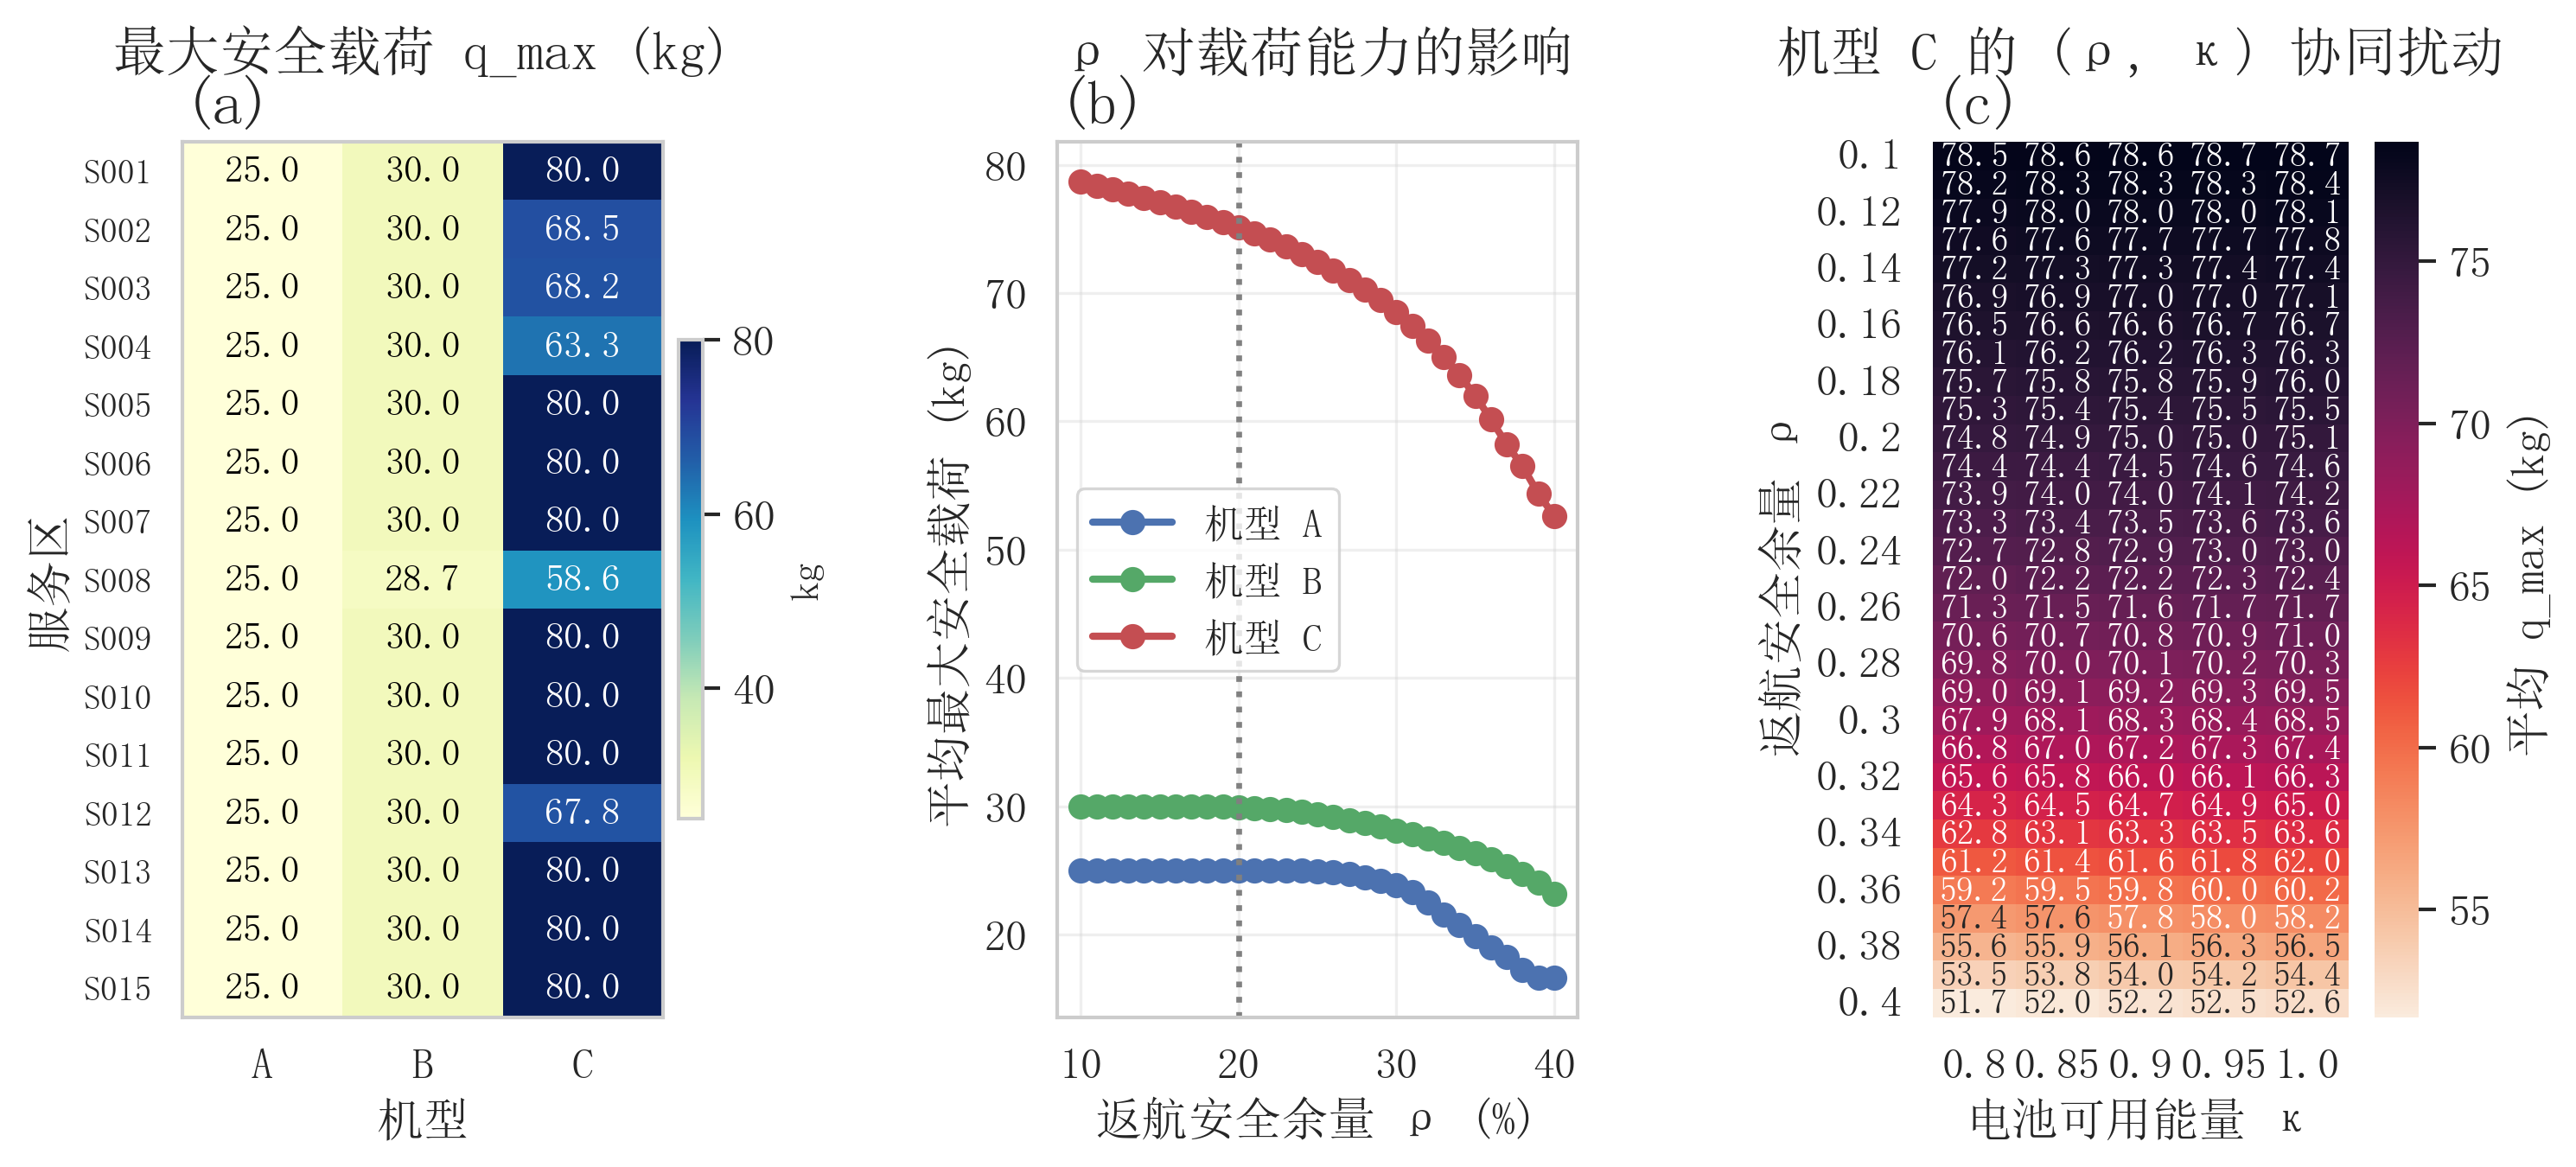
\includegraphics[width=0.95\textwidth]{figures/fig_q1_payload.png}
	\caption{最大安全载荷分布与双参数扰动}
	\label{fig:q1-payload}
\end{figure}

\subsection{货箱组批与优化}

在每个服务区内部，货箱不可拆分、不得跨服务区组批，需满足质量不超过最大安全载荷、体积不超过机型可用装载体积。同一服务区内的货箱只按（质量，体积）取值区分，取值相同的货箱在质量约束、体积约束、能耗与作业时间上完全等价，故先把货箱归并为\textbf{同质类}，再枚举“一个架次可以装哪几类各几件”的全部\textbf{架次模式}，最后在“各类货箱各取多少件”的\textbf{多重集状态}上做动态规划。状态为各类已运件数的多元组，每区货箱不超过 4 个同质类且每类件数有限，故状态空间不超过 $324$ 个，逐区求解耗时在毫秒量级，且给出的是该区在该机型下的\textbf{全局最优}组批。

为保证这一结论不依赖单一实现，本文用\textbf{两条独立路径}复核（结果见 \texttt{results/q1\_ilp\_gap.csv}）：其一为\textbf{指派式 0-1 整数规划}（变量为“箱 $i$ 放入架次 $j$”与“架次 $j$ 是否启用”，用 $y_{ij}\le u_j$、$u_j\le u_{j-1}$ 打破架次编号的置换对称），以最小化架次；其二为\textbf{集合划分整数规划}（先子集枚举出全部架次模式作为列，求恰好 $k$ 架次下的最小能耗），以最小化能耗。两条路径与动态规划在全部 $15\times3=45$ 个“服务区$\times$机型”组合上\textbf{逐行一致}；作为对照，若沿用降序首次适应（FFD）装箱，则在 45 个组合中有 2 个非最优（S007 与 S008 的 B 型，架次由 2 增至 3），对应能耗分别由 $3.427$ / $5.751$\,kWh 升至 $4.862$ / $8.165$\,kWh，全场景总能耗冗余约 $2.6\%$。

三种机型的全场景组批结果如表~\ref{tab:q1-batching}所示。

\begin{table}[htbp]
	\caption{三机型全场景组批结果对比}
	\label{tab:q1-batching}
	\centering
	\begin{tabular}{cccc}
		\toprule
		机型方案 & 往返架次数 & 总运输能耗（kWh） & 累计作业时间（h） \\
		\midrule
		全 A 型 & 52 & 112.371 & 24.82 \\
		全 B 型 & 35 & 68.470 & 15.47 \\
		全 C 型 & 18 & 74.061 & 9.40 \\
		\bottomrule
	\end{tabular}
\end{table}

由表可见三个指标存在明显的权衡：C 型以最少的架次（18）和最短的累计作业时间（9.40\,h）完成任务，但总能耗高于 B 型；B 型总能耗最低（68.470\,kWh）但架次增至 35、作业时间增至 15.47\,h；A 型在各指标上均劣于 B 型。据此本文推荐“大服务区用 C 型、小服务区用 B 型”的混合方案，以架次数为第一目标、能耗为第二目标：S001--S008 由 C 型承运（S001--S003 各村各需 2 架次，S004--S008 各 1 架次），S009--S015 由 B 型承运（各村 1 架次），共 18 架次、总能耗 63.180\,kWh、累计作业时间 9.173\,h——相对全 C 方案架次相同而能耗降低 $14.7\%$、时间缩短 $2.4\%$；相对全 B 方案架次减少 $48.6\%$、时间缩短 $40.7\%$ 而能耗还低 $7.7\%$，即在三个指标上同时不劣于两种单一机型方案。

进一步地，本文以架次上限为约束扫描出\textbf{帕累托前沿}（表~\ref{tab:q1-pareto}）。可见前沿非常平坦：架次由 18 增至 23（$+27.8\%$）仅换来总能耗由 $63.180$ 降至 $62.687$\,kWh（$-0.78\%$），代价是累计作业时间由 9.173\,h 增至 11.457\,h（$+24.9\%$）。这意味着在本题的能量参数下“多飞几趟以省电”几乎无效，架次数而非能耗才是运力规划的决定性指标，故取 18 架次方案为推荐方案。

\begin{table}[htbp]
	\caption{问题一组批方案的帕累托前沿}
	\label{tab:q1-pareto}
	\centering
	\small
	\begin{tabular}{ccccc}
		\toprule
		架次数 & 总能耗（kWh） & 累计作业时间（h） & 相对推荐方案能耗 & 相对推荐方案时间 \\
		\midrule
		\textbf{18} & \textbf{63.180} & \textbf{9.173} & --- & --- \\
		19 & 63.080 & 9.635 & $-0.16\%$ & $+5.0\%$ \\
		20 & 62.892 & 10.030 & $-0.46\%$ & $+9.3\%$ \\
		21 & 62.792 & 10.492 & $-0.61\%$ & $+14.4\%$ \\
		22 & 62.788 & 10.996 & $-0.62\%$ & $+19.9\%$ \\
		23 & 62.687 & 11.457 & $-0.78\%$ & $+24.9\%$ \\
		\bottomrule
	\end{tabular}
\end{table}

图~\ref{fig:q1-pareto}(a) 把表~\ref{tab:q1-pareto}的两支指标画在同一横轴上：总能耗随架次增加只是缓慢下行，累计作业时间却近似线性上升，两条曲线在 18 架次处张开的「剪刀口」直观说明了前沿为何平坦。(b) 给出各服务区自身的「架次–能耗」曲线族，纵轴取对数——不同服务区的单架次能耗量级相差很远，线性轴下小服务区的曲线会被压成一条线；可见同一服务区内换机型带来的能耗落差远大于同机型内增减架次的落差，这与前文「1 架 C 型可替代 2--3 架 B 型」的结构事实相符。(c) 则把 §5.3 的临界返航余量画成阶梯，架次数在 $\rho=0.2283$ 之前稳定在 18，此后逐级抬升。

\begin{figure}[htbp]
	\centering
	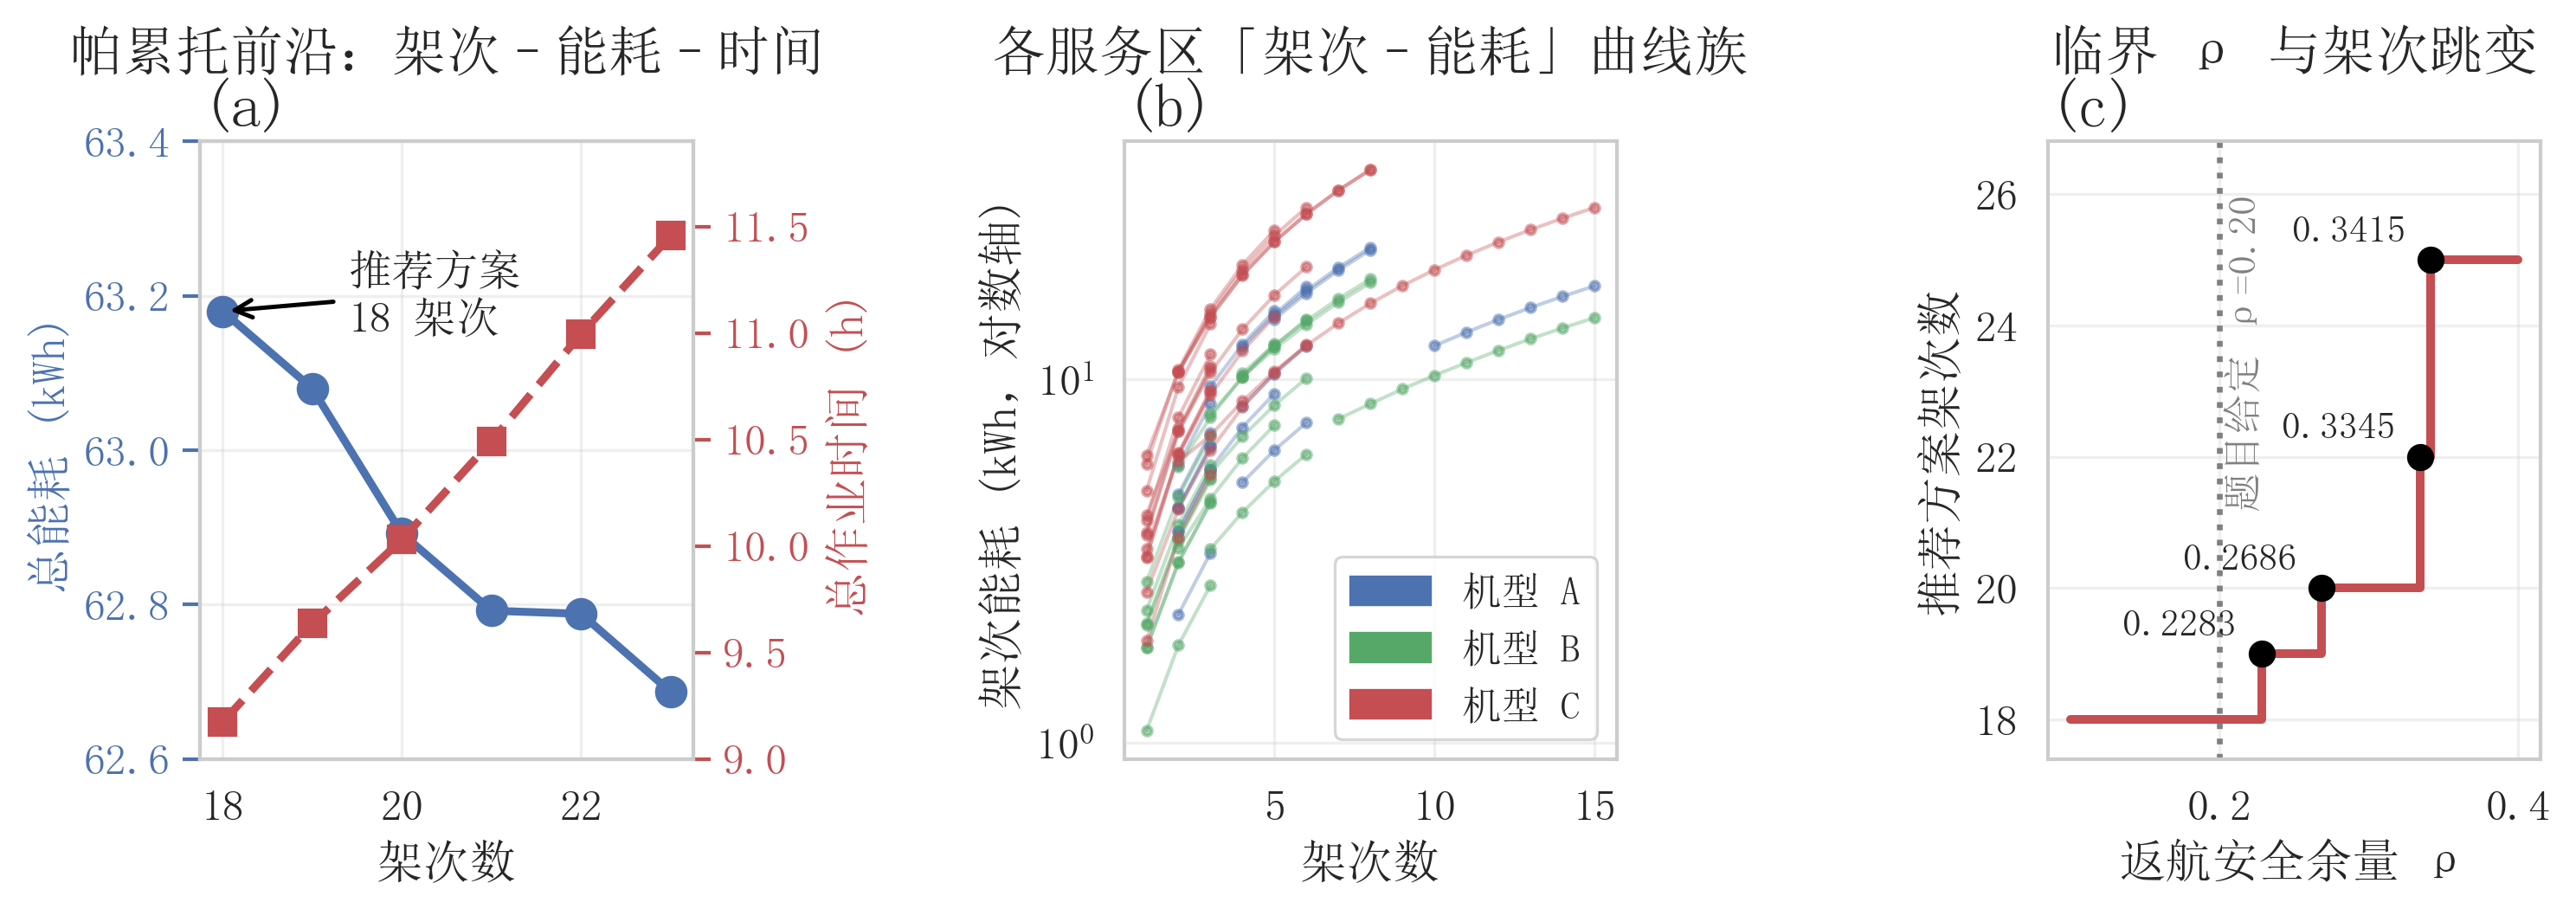
\includegraphics[width=0.95\textwidth]{figures/fig_q1_pareto.png}
	\caption{帕累托前沿、服务区曲线族与临界余量}
	\label{fig:q1-pareto}
\end{figure}

\subsection{返航安全余量的影响}

返航安全余量 $\rho_g$ 直接影响可用能量 $(1-\rho_g)E_g^{\mathrm{use}}$，进而改变最大安全载荷与组批结果。图~\ref{fig:q1-sens}给出了三种机型平均最大安全载荷随 $\rho$ 的变化。

\begin{figure}[htbp]
	\centering
	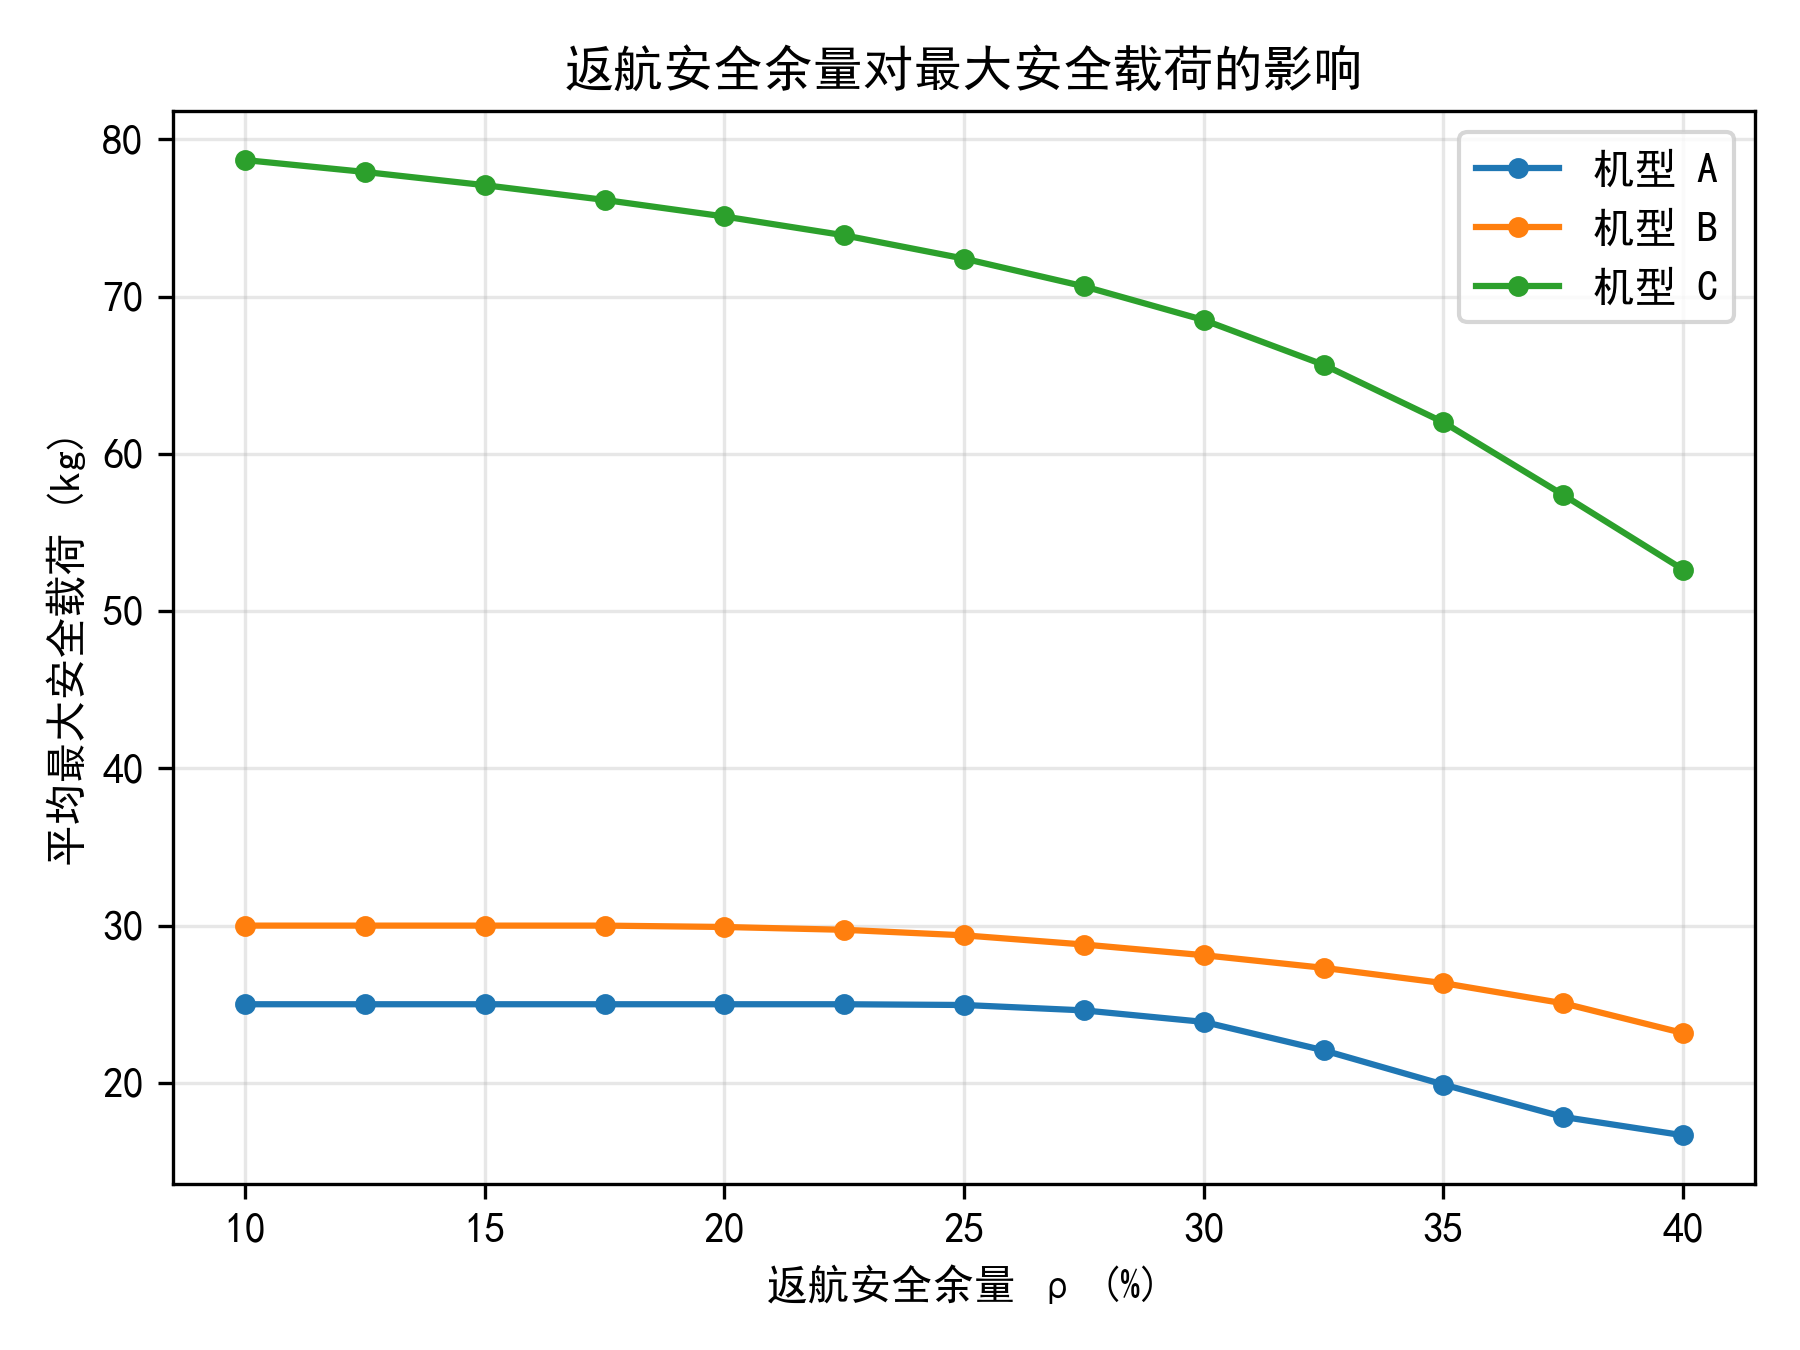
\includegraphics[width=0.62\textwidth]{figures/fig_q1_sensitivity.png}
	\caption{返航安全余量对最大安全载荷的影响}
	\label{fig:q1-sens}
\end{figure}

可见三型呈现三种不同的阶梯形态（同一条曲线亦见于图~\ref{fig:q1-payload}(b)）。A 型与 B 型在 $\rho$ 较小时是\textbf{平台}——$\rho\le0.20$ 时 A 型恒为 25.00\,kg、$\rho\le0.15$ 时 B 型恒为 30.00\,kg，说明此区间内二者的瓶颈是载质量上限而非能量，提高返航余量不损失运力。C 型则自始受能量约束，平均最大安全载荷由 $\rho=0.10$ 时的 78.68\,kg 单调降至 $\rho=0.40$ 时的 52.64\,kg（$\rho$ 每增大 10\% 平均下降约 8.7\,kg，与表~\ref{tab:sens}一致），且下降在 $\rho>0.30$ 后明显加速。

以总架次数为观测量对 $\rho$ 做二分定位，可得组批方案的\textbf{临界点}：$\rho=0.2283$ 时总架次由 18 跳至 19，此后 $0.2686$、$0.3345$、$0.3415$ 依次跳至 20、22、25 架次；当 $\rho$ 超过 $0.3513$ 时方案整体失效——此时最不利服务区 S008 对三种机型均已不可达。分机型看，S008 的作业可行性上界为 A 型 $0.2992$、C 型 $0.3510$、B 型 $0.3513$，即\textbf{率先失效的是航程最短、能量最小的 A 型}（$\rho>0.2992$ 后 A 型空载亦无法往返 S008），随后才是 C 型与 B 型。这意味着提高安全余量对运力的压缩不是均匀的：它先剥夺小型机的可达性、再压缩重载机的有效载荷，二者叠加使架次数阶梯式上升，安全性与运输效率需要在上述临界点之间权衡。
